\begin{center}
	\newcommand\maxt{2} % in [s]
	\newcommand\fSignal{2} % in [Hz]
	\newcommand\fTraeger{20} % in [Hz]
	\newcommand\Frequenzhub{5} % in [Hz]
	\pgfmathparse{\Frequenzhub/\fSignal}
	\xdef\Modulationsindex{\pgfmathresult}
	\pgfmathparse{1/\fSignal}
	\xdef\Periodendauer{\pgfmathresult}
	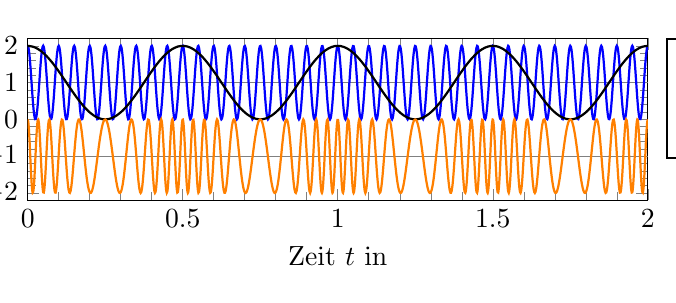
\begin{tikzpicture}[trim axis left, trim axis right]
	\begin{axis}[
	width=0.78\textwidth, height=0.3\textwidth,
	xlabel={Zeit $t$ in \si{\second}},
	ylabel={Amplitude in \si{\volt}},
	xmin=0, xmax=\maxt,
	xtick distance=0.5,
	minor x tick num=4,
	ymin=-2.2, ymax=+2.2,
	ytick distance=1,
	minor y tick num=4,
	legend style={cells={anchor=west}, legend pos=outer north east,},
	]
	\draw [gray] (0,+1) -- (\maxt,+1);
	\draw [gray] (0,-1) -- (\maxt,-1);
	\addplot [domain=0:{\maxt}, samples=1000, smooth, mark=none, thick, color=blue, solid] {cos(deg(2*pi*\fTraeger*x)) + 1};
	\addlegendentry{$U_{\text{T}} (t)$}
	\addplot [domain=0:{\maxt}, samples=100, smooth, mark=none, thick, color=black, solid] {cos(deg(2*pi*\fSignal*x)) + 1};
	\addlegendentry{$U_{\text{N}} (t)$}
	\addplot [domain=0:{\maxt}, samples=1000, smooth, mark=none, thick, color=orange, solid] {cos(deg(2*pi*\fTraeger*x + \Frequenzhub*sin(deg(2*pi*\fSignal*x)))) - 1};
	\addlegendentry{$U_{\text{FM}} (t)$}
	\end{axis}
	\end{tikzpicture}
\end{center}
